\subsection{积分的连续性质}

命题 8. --- 设 E 是 Hausdorff 的；设 \(\mu\) 是 X 上的一个测度。映射 \(\mathbf{f} \mapsto \int \mathbf{f} d\mu\) （ \(\mathcal{K}(\mathrm{X};\mathbf{E})\) 到 \(\widehat{\mathbf{E}}\) 中的；No.~3, 命题 7 的推论 1）是唯一的连续线性映射 \(\Phi\) ，它满足 \(\Phi(g \cdot \mathbf{a}) = \mu(g) \cdot \mathbf{a}\) 对每个向量 \(\mathbf{a} \in \mathbf{E}\) 及每个函数 \(g \in \mathcal{K}(\mathrm{X};\mathbf{C})\) 。

为证映射 \(f \mapsto \int f d\mu\) 的连续性，只需证明它在 \(\mathcal{K}(X, K; E)\) 上的限制对 X 的每个紧子集 K 都是连续的（TVS, II, §4, No.~4, 命题 5）。我们注意，若 E 的拓扑由半范数族 \((q_{\alpha})\) 定义，则 \(\mathcal{K}(X, K; E)\) 的拓扑由半范数族

\[
p _ {\alpha} (\mathbf {f}) = \sup _ {x \in K} q _ {\alpha} \bigl (\mathbf {f} (x) \bigr).
\]

定义。现在，设 h 是 X 到 \([0,1]\) 中的一个连续映射，具紧支集且在 K 上 \(h(x)=1\) ；由 No.~2 的命题 6，对每个函数 \(\mathbf{f}\in\mathcal{K}(\mathrm{X},\mathrm{K};\mathrm{E})\) 有

\[
q _ {\alpha} \left(\int \mathbf {f} d \mu\right) = q _ {\alpha} \left(\int h \mathbf {f} d \mu\right) \leqslant \int h (x) q _ {\alpha} (\mathbf {f} (x)) d | \mu | (x) \leqslant | \mu | (h) \cdot p _ {\alpha} (\mathbf {f})
\]

（诸 \(q_{\alpha}\) 已连续地延拓到 \(\widehat{\mathbf{E}}\) 上），这就证明了 \(\mathbf{f} \mapsto \int \mathbf{f} d\mu\) 的连续性。另一方面，按陈述中的记号，

\[
\int \left(g (x) \cdot {\bf a}\right) d \mu (x) = \mu (g) \cdot {\bf a}
\]

这依据 No.~1 的例 1 及 No.~2 的命题 2 应用于典范单射 \(\mathbf{C} \cdot \mathbf{a} \to \mathrm{E}\) 而得。此外， \(\mathcal{K}(\mathrm{X};\mathrm{E})\) 中由线性组合 \(\sum_{i} g_i \cdot \mathbf{a}_i\) （其中 \(\mathbf{a}_i \in \mathrm{E}\) ， \(g_i \in \mathcal{K}(\mathrm{X};\mathbf{C})\) ）所构成的子空间在 \(\mathcal{K}(\mathrm{X};\mathrm{E})\) 中稠密（§1, No.~2, 命题 5），这就完成了证明。

命题 9. --- 设 E 是 Hausdorff 的；设 f 是 X 到 E 中的一个具紧支集的连续映射。当空间 \(\mathcal{M}(\mathrm{X};\mathbf{C})\) 赋以严格紧收敛拓扑（§1, No.~10）时，映射 \(\mu \mapsto \int \mathbf{f} d\mu\) （ \(\mathcal{M}(\mathrm{X};\mathbf{C})\) 到 \(\widehat{\mathrm{E}}\) 中的）是唯一的连续线性映射 \(\Psi\) ，它满足 \(\Psi(\varepsilon_x) = \mathbf{f}(x)\) 对所有 \(x \in \mathrm{X}\) 。

对每个 \(\mathbf{z}' \in \mathrm{E}'\) ，

\[
\left\langle \int \mathbf {f} d \varepsilon_ {x}, \mathbf {z} ^ {\prime} \right\rangle = \int (\mathbf {z} ^ {\prime} \circ \mathbf {f}) d \varepsilon_ {x} = \mathbf {z} ^ {\prime} (\mathbf {f} (x)) = \langle \mathbf {f} (x), \mathbf {z} ^ {\prime} \rangle ,
\]

由此得 \(\int \mathbf{f} d\varepsilon_x = \mathbf{f}(x)\) 。此外我们知道，点测度所成之集在 \(\mathcal{M}(\mathrm{X};\mathbf{C})\) 中对严格紧收敛拓扑是全的（§2, No.~4, Th. 1 的推论 4）。于是问题归结为证明线性映射 \(u: \mu \mapsto \int \mathbf{f} d\mu\) 的连续性。为此，考虑线性映射 \(v: \mathbf{z}' \mapsto \langle \mathbf{f}, \mathbf{z}' \rangle\) （ \(\mathrm{E}'\) 到 \(\mathcal{K}(\mathrm{X};\mathbf{C})\) 中的），并证明 \(v\) 把一个等度连续子集 H （ \(\mathrm{E}'\) 的）映入 \(\mathcal{K}(\mathrm{X};\mathbf{C})\) 的一个严格紧子集中。因为若 K 是 \(\mathbf{f}\) 的支集，则诸函数 \(\langle \mathbf{f}, \mathbf{z}' \rangle\) （对 \(\mathbf{z}' \in \mathrm{H}\) ）的支集都含于 K；另一方面，这些函数构成一个等度连续集，且对每个 \(x \in \mathrm{X}\) ，诸 \(\mathbf{z}'(\mathbf{f}(x))\) 所成之集是有界的；于是我们的断言由 Ascoli 定理得出（GT, X, §2, No.~5, Th. 2 的推论 3）。现在，由 No.~1 的公式 (1) 可知， \(u\) 不是别的，正是 \(\mathcal{M}(\mathrm{X};\mathbf{C})\) 上的转置 \(^t v\) （代数意义的）的限制；因此其连续性由前述事实得出（TVS, IV, §1, No.~3, 命题 6）。

推论. --- 在命题 9 的假设与记号下，映射 \(\mu \mapsto \int \mathbf{f} d\mu\) 在正测度所成之集 \(\mathcal{M}_{+}(\mathrm{X})\) 上、或在 \(\mathcal{M}(\mathrm{X};\mathbf{C})\) 的一个淡有界子集 B 上的限制是淡连续的。

因为由 §1, No.~10 的命题 17 与 18 可知，在 \(\mathcal{M}_{+}(X)\) 上或在 B 上，由严格紧收敛拓扑诱导的拓扑与由淡拓扑诱导的拓扑相同。

\pandocbounded{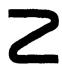
\includegraphics[keepaspectratio]{images/part001_df9b2198.jpg}}

然而，映射 \(\mu \mapsto \int \mathbf{f}d\mu\) 在整个 \(\mathcal{M}(\mathrm{X};\mathbf{C})\) 上对淡拓扑未必连续（习题 2）。

